\documentclass{ieeeaccess}
\usepackage{cite}
\usepackage{amsmath,amssymb,amsfonts}
\usepackage{algorithmic}
\usepackage{graphicx}
\usepackage{textcomp}
\usepackage{pdfpages}
\usepackage{url}
\usepackage[utf8]{inputenc}
\usepackage{array}
\usepackage{caption}
\newenvironment{human}{
    \begin{quote}
    \textbf{Human:}
}{\end{quote}}

\newenvironment{chatgpt}{
    \begin{quote}
    \textbf{LLMs:}
}{\end{quote}}

\newenvironment{Questions}{
    \begin{quote}
    \textbf{Questions:}
}{\end{quote}}

\newenvironment{Answers}{
    \begin{quote}
    \textbf{Answers:}
}{\end{quote}}
\def\BibTeX{{\rm B\kern-.05em{\sc i\kern-.025em b}\kern-.08em
    T\kern-.1667em\lower.7ex\hbox{E}\kern-.125emX}}
\begin{document}
\history{Date of publication xxxx 00, 0000, date of current version xxxx 00, 0000.}
\doi{10.1109/ACCESS.2017.DOI}

\title{ChoiceMaker: Empowering Sequential Model Optimization with Query Recommendations via Large Language Models}
\author{\uppercase{Feiran (Alex) Qin}\authorrefmark{1}}
\address[1]{Computer Science Department, North Carolina State University, Raleigh, NC 27695, USA}


\tfootnote{
    %This paragraph of the first footnote will contain support 
% information, including sponsor and financial support acknowledgment. For 
% example, ``This work was supported in part by the U.S. Department of 
% Commerce under Grant BS123456.''
}

\markboth
{Author \headeretal: Preparation of Papers for IEEE TRANSACTIONS and JOURNALS}
{Author \headeretal: Preparation of Papers for IEEE TRANSACTIONS and JOURNALS}

\corresp{
    Corresponding author: Feiran (Alex) Qin (e-mail: fqin2@ncsu.edu).
    }

\begin{abstract}
    Choice is not only important in human lives but also crucial in software engineering. In the CSC 791 Automated Software Engineering class, we are tasked with implementing a Sequential Model Optimizer that uses Root Mean Square Deviation (RMSE) as the evaluation metric. This paper proposes a novel approach that enhances Sequential Model Optimization with Query Recommendations through the use of Large Language Models (LLMs). Initially, we compare RMSE methods with those of LLMs. Subsequently, we evaluate the effectiveness of LLMs across various models with differing numbers of tokens, the scalability of few-shot learning, and the costs associated with self-hosted and commercial models. Although LLMs did not perform as well as RMSE in the SMO algorithm, they demonstrated a advantage in terms of interpretability.
\end{abstract}

\begin{keywords}
Software Engineering, Large Language Models, Sequential Model Optimization
\end{keywords}

\titlepgskip=-15pt

\maketitle

\section{Introduction}
\label{sec:introduction}
\PARstart{C}{hoice} making is a central concern in software engineering. According to Long et al.\cite{10352439}, engineers typically spend a third of their time on activities such as planning, coding, and testing. In software engineering, over half of this time is devoted to tasks related to making choices, such as planning, analysis, and testing, which are critical for ensuring software reliability. As software projects scale, the volume of data and parameters increases significantly. The number of control parameters in a software package tends to grow linearly over time, whereas human understanding of these parameters grows at a sub-linear rate\cite{10.1145/2786805.2786852}. It is challenging for humans to consistently make optimal decisions, and poor choices can lead to disastrous outcomes. For instance, 30\% of cloud computing errors are attributed to misconfigurations\cite{yy}, and even more troubling, 59\% of severe performance bugs arise from inadequate configurations—highlighting that poor decision-making is a major threat to software quality\cite{10.1145/2961111.2962602}. Automating decision-making in software has emerged as a significant yet underappreciated success story, with AI tools proving highly effective in predicting the outcomes of different choices\cite{9734271}.

In the CSC 791 Automated Software Engineering course, Dr. Menzies introduced Sequential Model Optimization using Root Mean Square Deviation (RMSE) as the evaluation metric for decision-making. However, RMSE often fails to capture the true meaning of the data and can be misled by outliers.

In this work, we propose a novel approach that enhances Sequential Model Optimization with Query Recommendations using Large Language Models (LLMs). We address several key technical challenges, including:
\begin{itemize}
  
 

        \item \textbf{How to choose the best prompts balancing accuracy and cost?}
        To enhance the accuracy of LLMs and obtain the desired response, we consider several strategies: zero-shot prompts, few-shot prompts, and fine-tuning. The costs and benefits of these methods increase respectively. The cost-effectiveness ratio varies depending on multiple factors such as the dataset, the model, and the optimization objectives. We aim to develop a quantitative paradigm to guide prompt tuning for datasets of similar sizes.
        
        \item \textbf{How to evaluate the output of LLMs without ground truth?}
        Like the previous Sequential Model Optimization (SMO) method using RMSE, evaluating the outputs of LLMs is challenging in the absence of ground truth. This difficulty persists whether the outputs are feasible or present in the dataset. We seek to establish methods to assess LLM outputs without ground truth, or alternatively, to discover heuristic rules that can retroactively adjust the prompt to enhance accuracy.
        
        \item \textbf{Which model to choose considering privacy, cost, and accuracy?}
        Numerous models are available, ranging from open-source options like llama2 to commercial variants such as ChatGPT, including versions with different token counts such as 8b, 13b, and 33b. Open-source models, which are easier to self-host, offer greater privacy, particularly with sensitive or commercial data. Although commercial models typically offer superior performance, the gap between them and open-source alternatives is diminishing. By assessing different models’ capabilities in the selection task, we hope to elucidate the performance disparities between models and track the evolution of their capabilities over time.
 
\end{itemize}

\begin{figure*}[ht]
    \centering
    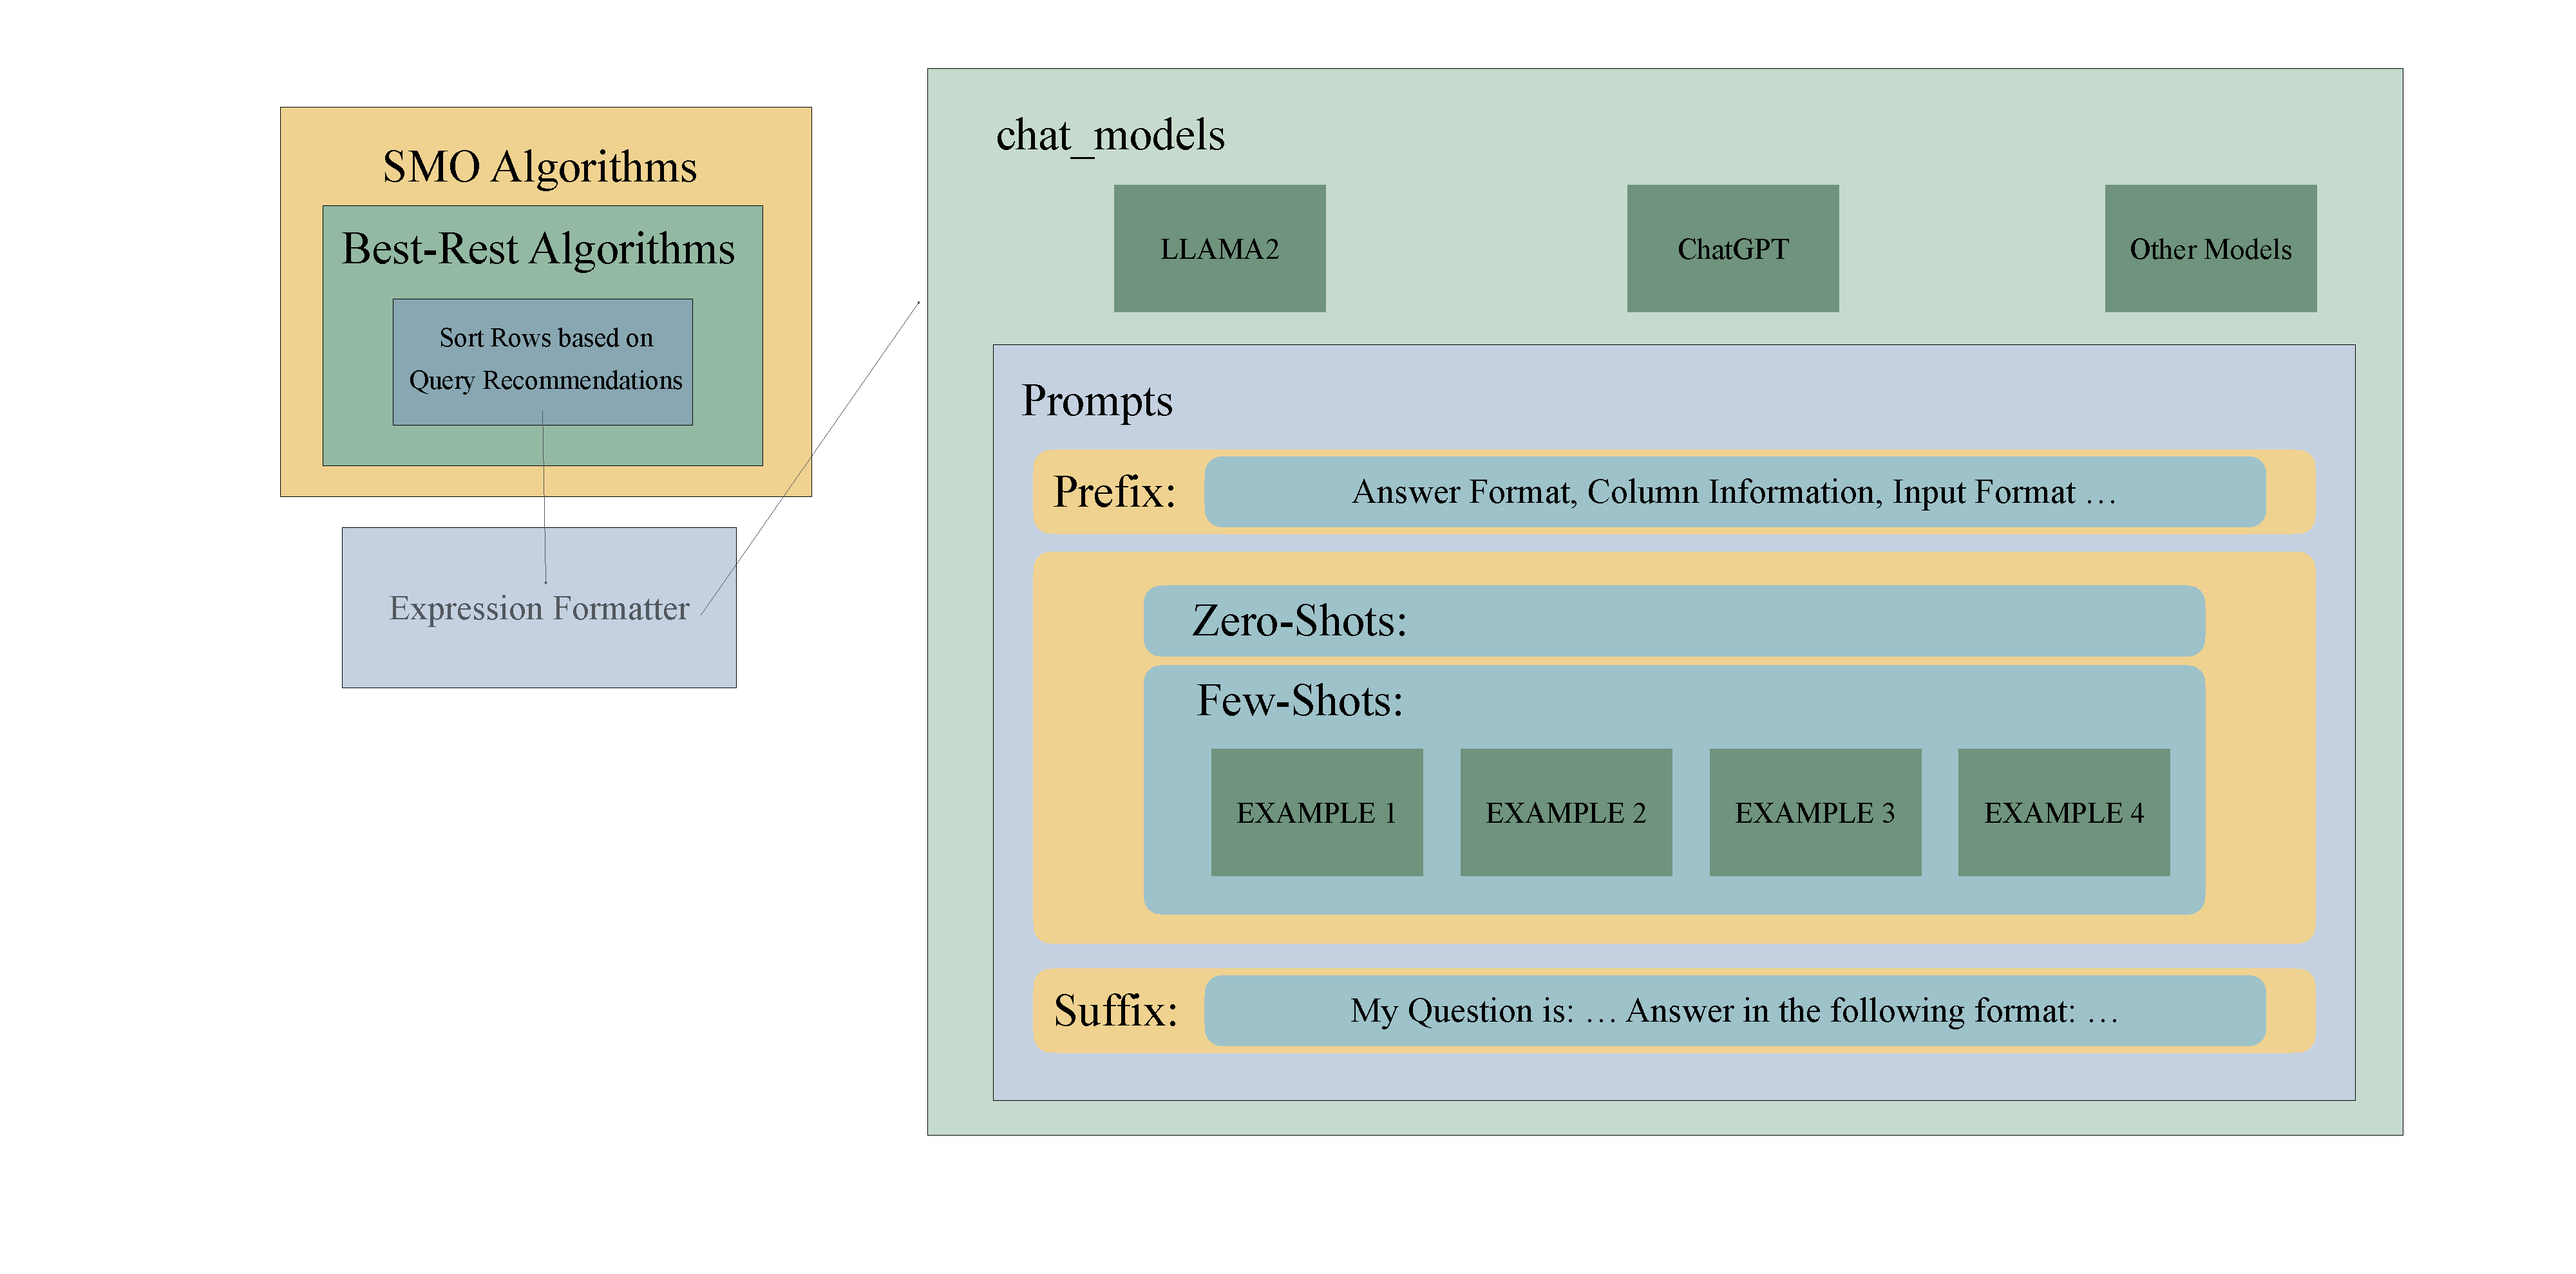
\includegraphics[page=1,width=\textwidth]{intro.pdf}
    \caption{An overview of ChoiceMaker} \label{fig.1}
  \end{figure*}


  The ChoiceMaker consists of three parts, as shown in Fig.\ref{fig.1}:
  \begin{itemize}
  
  \item \textbf{A modification to the SMO algorithm that sorts rows based on query recommendations provided by LLMs.}
  To maintain ease of evaluation and ensure accuracy, we have made minimal changes to the original SMO algorithm. Specifically, we replaced the original sorting mechanism with one that incorporates RMSE to evaluate the effectiveness of query recommendations.
  
  \item \textbf{An expression formatter}
  that formats queries specifically for the LLMs, particularly the data rows used for sorting. It includes a regular expression to extract information from the outputs of the LLMs, streamlining the integration of these outputs into the SMO process.
  
  \item \textbf{An LLM client built on the LangChain framework.}
  We utilized the LangChain library to facilitate the development of our LLM client. LangChain provides an abstraction layer for calling APIs across different language models, enabling the instantiation of various large predicate models. This abstraction allows for easy switching between evaluation models, such as llama2 and ChatGPT. Our prompts include prefixes, examples, and suffixes. In the prefix, we carefully specify the answer format, column information, and input format for the prompt. If few-shot tuning is desired, we can provide LLMs with several optional sets of examples, ranging from ${0,4,8}$ to assess the impact of training extent on performance. Each set includes samples and factual responses. The suffix contains the final question, typically a preference choice, and reiterates the answer format to ensure that responses can be parsed using the designated regular expression. In cases of suboptimal performance, we adjust the prompts manually, for example, by adding motivational phrases like "we'll tip you" or defining the identity of the LLMs more precisely.
  
  \end{itemize}

  This paper offers the following contributions:
  \begin{itemize}
    \item A novel approach that integrates Sequential Model Optimization with Query Recommendations using Large Language Models (LLMs).
    \item An evaluation of the scalability of few-shot learning.
    \item A demonstration of the limitations and unique advantages of LLMs in optimizing software engineering choices.
    \item An exploration of the evolution of LLMs, illustrating their growing impact and refinement over time.
    \end{itemize}
  
  The organization of this paper is as follows: Section \ref{sec:background} provides background information on the issue of decision-making in software engineering. Section \ref{sec:algorithms} details the algorithms employed in our study. Section \ref{sec:methods} outlines the methods used for implementing our approach. Section \ref{sec:results} presents the findings from our experiments. Section \ref{sec:discussion} discusses the implications of these results. Finally, Section \ref{sec:conclusion} concludes the paper and suggests directions for future research.

\section{Background}
\label{sec:background}
\subsection{Sequential Model Optimization with Root Mean Square Deviation (RMSE)}
Sequential Model Optimization (SMO) is a method for optimizing the performance of a model by iteratively selecting the best model from a set of models. The RMSE is a measure of the difference between the predicted value and the actual value. The RMSE is calculated as the square root of the average of the squared differences between the predicted value and the actual value. The RMSE is a measure of the accuracy of a model, with lower values indicating better performance. The RMSE is often used as an evaluation metric in machine learning tasks, such as regression and classification. In the context of SMO, the RMSE is used to evaluate the performance of a model and select the best model from a set of models. The RMSE is calculated for each model in the set, and the model with the lowest RMSE is selected as the best model. The RMSE is used to guide the selection of models in the SMO process, with the goal of finding the model that performs best on the given task.

The RMSE formula is given by:

\begin{equation}
    \text{RMSE} = \sqrt{\frac{1}{n} \sum_{i=1}^n ( \lvert h_i - c_i \rvert)^2}
\end{equation}

where:
\begin{itemize}
    \item $n$ is the total number of observations or data points.
    \item $h_i$ represents the observed value for each data point $i$, derived from col.heaven. The "Heaven Value" (col.heaven) is a human-specific value that users can specify a \{0,1\} value to represent their preferences. For instance, if someone wants a car that's both fast and light, they could set the horsepower col.heaven to 1 and the weight col.heaven to 0 in an automotive database.
    \item $c_i$ is the calculated or expected value for each data point $i$, obtained from the expression col.norm(self.cells[col.at]). $c_i$ is a normalized value that fits within the range of 0 to 1.
    \item $(h_i - c_i)^2$ computes the square of the difference between the observed value and the calculated value for each data point.
    \item $\sqrt{\frac{1}{n} \sum_{i=1}^n (\cdot)}$ takes the square root of the average of these squared differences, yielding the RMSE, a measure of the magnitude of deviation between observed and calculated values.
\end{itemize}

The SMO algorithm is a method for optimizing the performance of a model by iteratively selecting the best model from a set of models. The SMO algorithm works as follows:

\begin{enumerate}
    \item \textbf{Shuffling:} The data rows are shuffled initially to randomize their order.
    \item \textbf{Initial Evaluation:} The method prints the root mean square deviation (d2h) for the first 6 and first 50 rows post-shuffling, providing baseline performance metrics. The choice of row count can be adjusted, noting that this depends on computational resources, Determined by variables \texttt{budget0} and \texttt{budget}.
    \item \textbf{Data Partitioning:} Rows are split into two groups, \texttt{lite} and \texttt{dark}, based on a specified budget threshold (\texttt{budget0}).
    \item \textbf{Iterative Evaluation and Selection:}
        \begin{itemize}
            \item The method iteratively processes the \texttt{lite} group by partitioning it further into \texttt{best} and \texttt{rest} segments and evaluating them.
            \item A selection process takes place where certain rows are moved from the \texttt{dark} group to the \texttt{lite} group based on evaluation results.
            \item Statistical outcomes and best-performing rows from these evaluations are recorded.
        \end{itemize}
    \item \textbf{Output:} The method returns two dictionaries, \texttt{stats} (containing mid-point evaluation data of selected rows) and \texttt{bests} (containing the best-performing rows in each iteration).
\end{enumerate}

The process of selection is based on the RMSE, which is calculated for each row in the \texttt{lite} group. The RME is used to evaluate the performance of each row, and the best-performing rows are selected for further evaluation. The SMO algorithm iteratively selects the best-performing rows and evaluates them to find the optimal solution. The Best-Rest selection works as follows:

\begin{itemize}
    \item Initially, the function sorts the input rows based on a specific metric calculated by the \texttt{d2h} method, which presumably stands for "distance to heaven." This metric quantifies how closely each row aligns with a predefined ideal or benchmark, referred to as "heaven"
    \item \textbf{Partitioning Rows into 'best' and 'rest'}:
    The function iterates through the sorted rows and divides them into two groups. The division is based on a specified number (want).
    The first want rows (those closest to heaven) are added to the best list, implying that these rows meet or exceed a certain threshold of desirability or fit.
    The remaining rows are added to the rest list, indicating that while they are still valid, they do not match the criteria as closely as those in the best group.
\end{itemize}

\subsection{Large Language Models (LLMs)}

Large Language Models (LLMs) are a class of machine learning models that are trained on large amounts of text data. LLMs are capable of generating human-like text and have been used in a variety of natural language processing tasks, such as text generation, translation, and summarization. LLMs are typically trained on large datasets of text, such as books, articles, and websites, and are able to learn the statistical patterns in the data to generate text that is coherent and grammatically correct. LLMs are typically trained using deep learning techniques, such as neural networks, and are able to learn complex patterns in the data to generate text that is indistinguishable from human-written text. LLMs have been shown to be effective in a variety of natural language processing tasks, and have been used in a variety of applications, such as chatbots, language translation, and text summarization.

The most common LLMs are based on the transformer architecture, which was introduced by Vaswani et al. in 2017. The transformer architecture is a deep learning model that is based on self-attention mechanisms, which allow the model to focus on different parts of the input data to generate output. The transformer architecture has been shown to be effective in a variety of natural language processing tasks, and has been used in a variety of applications, such as language translation, text generation, and text summarization. The transformer architecture has been used to train large language models, such as GPT-2\cite{radford2019language}, GPT-3\cite{brown2020language}, and BERT\cite{devlin2018bert}, which have been shown to be effective in a variety of natural language processing tasks.

Popular large language models currently in use are Commercially models such as ChatGPT-4\cite{chatgpt4} and Claude-AI\cite{claudeai} and Open-source models that can be deployed by oneself like LLaMA v3\cite{llama} and Gemma\cite{gemma}.


Tawosi et al.\cite{Tawosi_2023} explores the use of search-based software engineering (SBSE) techniques to optimize the number and combination of examples provided to large language models (LLMs) for few-shot learning. This optimization aims to enhance the models' ability to estimate story points in agile software development tasks. Saparov et al.\cite{saparov2023testing} explores the ability of large language models (LLMs) to perform deductive reasoning using out-of-distribution (OOD) examples. It specifically assesses the LLMs' ability to generalize from simpler proofs to more complex ones across different dimensions: depth, width, and compositional complexity of proofs. 

New perspectives have been brought to traditional machine learning algorithms and software engineering design by LLMs. Assessing the capabilities of LLMs in these areas is still a challenge, especially with new models emerging constantly. The latest version of Llama V3 was released just days ago. Therefore, this paper hopes to replace RMSE with LLMs for providing recommendations on SMO algorithms and conduct an assessment based on that foundation. These assessments will not only evaluate the capabilities of various models but also include evaluations of few-shot learning's scalability.

\section{Algorithms}
\label{sec:algorithms}

This section addresses two primary concerns:
A. The potential benefits of replacing RMSE with a large language model,
B. Effective strategies for prompting a large language model to achieve desired outcomes.

\subsection{RMSE and LLM}
Root Mean Squared Error (RMSE) has several limitations:
\begin{itemize}
\item RMSE does not comprehend the real meaning of data and can be misled by outliers.
\item RMSE measures the magnitude of deviation between observed and predicted values, but does not indicate the direction of this deviation.
\item While RMSE is a good indicator of a model's accuracy, with lower values signifying better performance, it does not necessarily reflect the overall quality of the model.
\end{itemize}
Although RMSE effectively represents the deviation in data, it lacks insight into the actual significance of the data, leading to selections that may be theoretically optimal but not practically feasible. Additionally, the quality of initial selections in the SMO algorithm significantly influences the learning process and the efficacy of subsequent selections and filtering.

To address these issues, this paper proposes the integration of large language models (LLMs) into the "best-rest" selection strategy of the SMO algorithm. Traditionally, this strategy involves sorting data based on RMSE to identify a subset of "best" samples while relegating the rest. To mitigate concerns about overfitting, particularly with small local samples, LLMs are employed to enhance the sorting process.

The modified "Best-Rest" selection algorithm operates as follows:

The algorithm begins by sorting according to user preferences via a large language model. The user's preference is integrated into the prompt, which is then processed by the LLM. Instead of requiring the LLM to provide a complete ranking, the model is prompted with comparative queries like "Is A better than B?", and its responses are used as sorting keys.

The rationale for not relying on large prediction models to directly produce sorted results, but rather using a combination of incremental comparison and sorting algorithms, includes the following considerations. Firstly, while the SMO algorithm may involve fewer rows in a single "Best-Rest" selection cycle, larger datasets significantly increase the number of rows needing sorting. Many models have constraints, such as the 4,096-character limit per prompt in the web-based ChatGPT. Moreover, large inputs can degrade decoder performance, particularly as most large prediction models utilize substantial batch sizes and parallel processing. Additionally, in models with limited long-term memory (e.g., llama2:8b), extensive inputs can compromise sorting effectiveness. These challenges were identified during preliminary experiments, leading to the adoption of an incremental comparison and sorting approach to ensure universality and accuracy of the algorithm.
\subsection{Prompting LLMs}
In this section, we discuss the challenges and design trade-offs encountered when crafting prompts for large language models (LLMs). These considerations are crucial for maximizing the effectiveness of LLMs in our application.

\subsubsection{Identity Specification and Data Information}

To improve the relevance and personalization of the LLM responses, we initially set the identity of the LLM to match the context of the dataset. For example, in a dataset related to automobiles, the LLM assumes the role of an exceptional car sales consultant. This pre-set identity helps tailor the LLM’s responses to be more contextually appropriate.

Additionally, providing detailed column information within the prompts has proven to be of paramount importance. Here are examples demonstrating how this information is utilized in prompts with the llama2:13b model:

\begin{human}
... Here are some data: \\
Clndrs,Volume,HpX,Model,origin,Lbs-,Acc+,Mpg+ \\
8,304,193,70,1,4732,18.5,10 \\
8,360,215,70,1,4615,14,10 \\
Which is faster? ...
\end{human}

\begin{chatgpt}
... The Volume model is the way to go! ...
\end{chatgpt}

\begin{human}
[Previous Prompts] ... Number of Cylinders, Cylinder capacity, Horsepower, Model of the car, Origin of the car, Weight of the car, Acceleration, Miles per gallon ...
\end{human}

\begin{chatgpt}
... with its impressive 70 horsepower engine and a svelte weight of only 14 pounds ...
\end{chatgpt}

As depicted in Figure \ref{fig.2}, integrating identity specifications and detailed data information into prompts significantly enhances the response quality of LLMs. While LLMs like llama2 can infer meanings from column headers, their ability to utilize all provided columns effectively can vary. More advanced models, such as LLaMA 3, show marked improvements in utilizing this information compared to their predecessors.

\begin{figure}[ht]
\centering
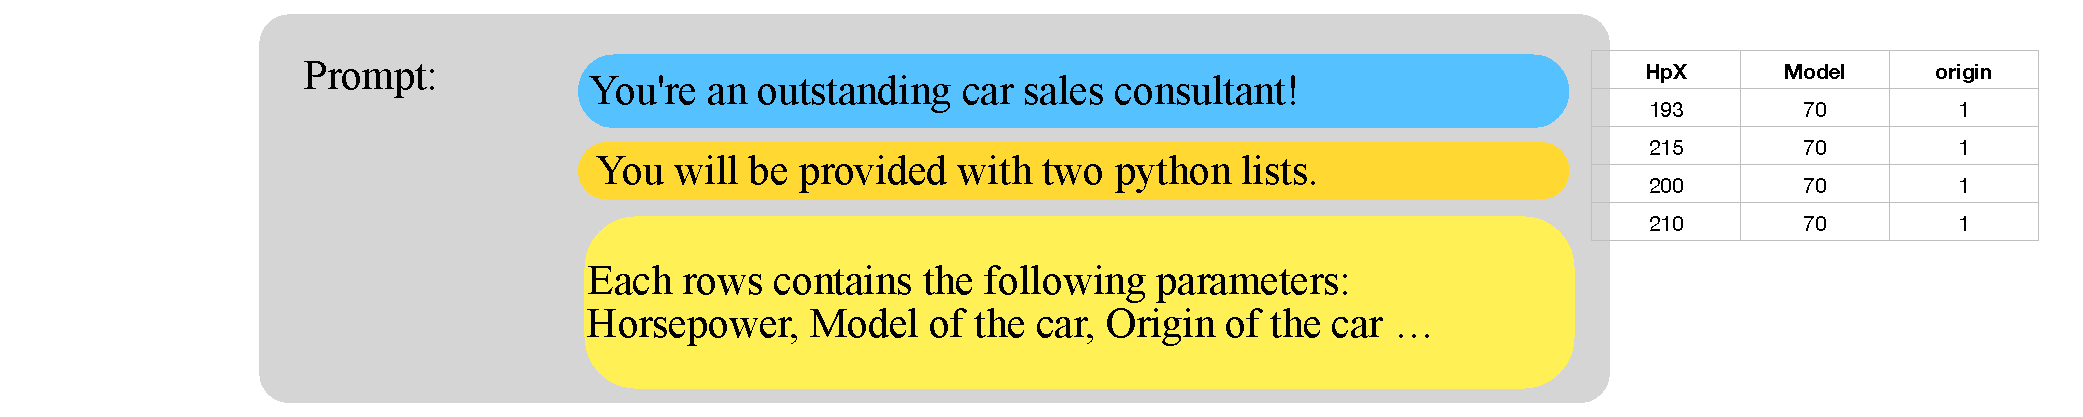
\includegraphics[page=1,width=0.5\textwidth]{llm1.pdf}
\caption{Integration of identity specifications and data information into prompts.} % 添加标题
\label{fig.2}
\end{figure}

The examples demonstrate that providing comprehensive data details leads LLMs to consider a broader array of factors during their processing. However, the degree to which each column is utilized depends heavily on the model’s capabilities.

\subsubsection{Answer Format}

One of the significant challenges we encountered involves ensuring that LLMs respond according to a pre-specified format, despite the capabilities provided by the \texttt{llama.cpp} library. This library includes GBNF (GGML BNF) functionality, which allows for the definition of formal grammars to standardize model outputs. For example, GBNF can be used to enforce that the model's output is in valid JSON format or to limit responses strictly to emojis\cite{llamacpp}. However, this functionality is not universally applicable, especially not with commercial models or those not integrating the \texttt{llama.cpp} framework.

To manage the formatting of responses, we devised prompts designed to direct the models' output structure as precisely as possible. An example prompt we implemented is as follows: "If the first list has [preference], you should answer 'A.' If the second list has more [preference], you should answer 'B.' If both lists have the same [preference], you should answer 'Same.'"

Despite these efforts, ensuring consistent adherence to the specified format remains a challenge. Language models do not always respond as expected. To mitigate this, we have reinforced format constraints through careful crafting of both the prefix and suffix in our prompts, employing capitalization to highlight essential elements. This method helps improve the likelihood that responses adhere to the desired format, although it is not foolproof.

\subsubsection{Few-shot Learning}

Few-shot learning for Large Language Models (LLMs) capitalizes on the model's ability to quickly adapt to new tasks or understand new types of queries with very limited examples. This method utilizes the extensive knowledge these models have accumulated during their initial training phase, enabling them to generalize from just a few examples presented at inference time\cite{brown2020language}.

We implement few-shot learning by incorporating specific ground-truth examples from our dataset directly into the prompts. For instance:

\begin{Questions}
"Which car has more horsepower, A or B or is it the Same? A: [4, 140, 86, 82, 1, 2790, 15.6, 30], B: [4, 91, 67, 82, 3, 1965, 15.7, 30]?"
\end{Questions}

\begin{Answers}
"A"
\end{Answers}
\begin{Questions}
"Which car has more cylinders, A or B or is it the Same? A: [4, 140, 86, 82, 1, 2790, 15.6, 30], B: [4, 91, 67, 82, 3, 1965, 15.7, 30]?"
\end{Questions}

\begin{Answers}
"Same"
\end{Answers}

We have also experimented with using abstract concepts rather than specific details as prompts, such as asking about reliability instead of particular models or manufacturing methods. However, this approach did not yield improvements, and controversies regarding the selection of correct answers persisted.

In summary, we leverage example-based prompts for few-shot learning, enabling us to assess the differences between zero-shot and {2, 4, 8}-shot learning configurations in subsequent evaluations.

    \section{Methods}
    \label{sec:methods}
    \subsection{Data}
    For our primary dataset, we selected the Auto93 dataset, commonly known as the "Auto MPG" dataset. Sourced from the UCI Machine Learning Repository, this dataset is frequently utilized for regression analysis tasks in machine learning. It comprises data from cars of the 1970s and early 1980s, with a focus on fuel consumption\cite{auto_mpg_1993}.

    The key features of the Auto93 dataset are outlined in Table \ref{tbl.1}:

    \begin{table*}[h!]
        \centering
        \begin{tabular}{|>{\raggedright\arraybackslash}p{3cm}|>{\raggedright\arraybackslash}p{9cm}|}
        \hline
        \textbf{Feature} & \textbf{Description} \\
        \hline
        MPG & The target variable, representing the fuel efficiency in miles per gallon. \\
        \hline
        Cylinders & The number of cylinders in the car's engine. \\
        \hline
        Displacement & The engine displacement, measured in cubic inches. \\
        \hline
        Horsepower & The power output of the engine, measured in horsepower. \\
        \hline
        Weight & The vehicle's weight in pounds. \\
        \hline
        Acceleration & The time (in seconds) it takes for the vehicle to accelerate from 0 to 60 mph. \\
        \hline
        Model Year & The year of the car model. \\
        \hline
        Origin & The origin of the car's manufacturer. \\
        \hline
        Car Name & The make and model of the car. \\
        \hline
        \end{tabular}
        \caption{Description of the Auto93 dataset features}
        \label{tbl.1}
        \end{table*}

        To increase the diversity of our data, we additionally analyzed the Wine Quality dataset. This dataset relates to red and white variants of Portuguese "Vinho Verde" wine, and it's utilized to predict wine quality on a scale from 0 (very bad) to 10 (excellent)\cite{cortez2009}. The features of this dataset are summarized in Table \ref{tbl.2}:

    \begin{table*}[h!]
        \centering
        \begin{tabular}{|>{\raggedright\arraybackslash}p{4cm}|>{\raggedright\arraybackslash}p{8cm}|}
        \hline
        \textbf{Feature} & \textbf{Description} \\
        \hline
        Fixed acidity & Measures the amount of tartaric acid in the wine, which is crucial for the color, balance, and taste of the wine. \\
        \hline
        Volatile acidity & The amount of acetic acid in wine, which at too high of levels can lead to an unpleasant vinegar taste. \\
        \hline
        Citric acid & Found in small quantities, citric acid can add 'freshness' and flavor to wines. \\
        \hline
        Residual sugar & The amount of sugar remaining after fermentation stops, it's rare to find wines with less than 1 gram/liter and wines with greater than 45 grams/liter are considered sweet. \\
        \hline
        Chlorides & The amount of salt in the wine. \\
        \hline
        Free sulfur dioxide & The free form of SO\(_2\) exists in equilibrium between molecular SO\(_2\) (as a dissolved gas) and bisulfite ion; it prevents microbial growth and the oxidation of wine. \\
        \hline
        Total sulfur dioxide & Amount of free and bound forms of S02; in low concentrations, SO2 is mostly undetectable in wine, but at free SO2 concentrations over 50 ppm, SO2 becomes evident in the nose and taste of wine. \\
        \hline
        Density & The density of wine is close to that of water depending on the percent alcohol and sugar content. \\
        \hline
        pH & Describes how acidic or basic a wine is on a scale from 0 (very acidic) to 14 (very basic); most wines are between 3-4 on the pH scale. \\
        \hline
        Sulphates & A wine additive which can contribute to sulfur dioxide gas (S02) levels, wich acts as an antimicrobial and antioxidant. \\
        \hline
        Alcohol & The percent alcohol content of the wine. \\
        \hline
        Quality (target) & Score between 0 and 10. \\
        \hline
        \end{tabular}
        \caption{Features of the Wine Quality dataset}
        \label{tbl.2}
        \end{table*}
    
        While it would be beneficial to expand our analysis to include additional datasets, our current study is constrained by limited computational resources and the relatively low efficiency of our algorithms. These limitations restrict the number of datasets we can feasibly analyze within a given timeframe. For a more comprehensive understanding of these challenges and their implications for our research, further details are provided in the discussion section (see Section \ref{sec:discussion}).

        \subsection{Experiment Set Up}

        We have structured our evaluation process to utilize large language models, as detailed in Table \ref{tbl.3}. Our key experiments focus on assessing the performance of the LLaMA 3:8B model across various testing scenarios.
        
        \subsubsection{Comparison between SMO with RMSE and SMO with LLMs}
        
        The cornerstone of our experimental design is to compare the effectiveness of the Sequential Model Optimization (SMO) algorithm with and without the integration of Large Language Models (LLMs), and against the traditional use of RMSE alone. For this purpose, we utilized the LLaMA 3 model to guide the SMO algorithm in processing data from both the Auto93 and Wine Quality datasets. We applied RMSE as our evaluation metric, conducted 10 rounds of randomized experiments, and recorded the RMSE values for each trial. This allowed us to compare the average RMSE values when employing SMO with just RMSE and when using SMO augmented by LLMs. Our experiments consistently employed an 8-shot approach in the few-shot learning setting.
        
        \subsubsection{Comparative testing with varying numbers of few-shot instances}
        
        In this series of tests, we aim to assess the impact of different few-shot learning configurations on model performance. We will experiment with a range of setups, from zero-shot learning (no examples provided) to more extensive few-shot scenarios involving zero, four, eight examples per class. The primary dataset for these experiments is Auto-93. We will evaluate the models based on the average Root Mean Squared Error (RMSE) obtained from at least 5 random trials, aiming to determine how varying the number of few-shot examples influences the accuracy of the results.
        
        \subsubsection{Cost-performance considerations for various large language models}
        
        This experiment is designed to analyze the cost-performance balance of various large-scale language models, including ChatGPT-4, LLaMA3, and the 13B configurations of LLaMA2. We will assess these models' performance based on accuracy, processing speed, and computational resource demands. The evaluation will be conducted using the Auto93 dataset, employing an 8-shot learning approach to gauge each model's efficacy under comparable conditions.

        \subsubsection{Experimental Settings}

        Due to the limited computational resources and inefficiencies in our sorting algorithms discussed further in the discussion section (see Section \ref{sec:discussion}), our experimental design includes some specific constraints. To manage these limitations while maintaining the integrity of our experimental analysis, we will conduct a minimum of five random trials for each experiment.

        For the datasets used in our experiments, namely Auto 93 and Wine Quality, we have set specific budget parameters. The budget allocations are defined as follows: budget0 is set at 4, budget at 16, and some at 0.5. These settings are carefully chosen to balance between computational feasibility and the need for reliable data to support our findings. These budgetary constraints are intended to optimize our resource allocation while allowing us to conduct meaningful experiments within the confines of available resources.



\subsection{Evaluation metrics}
We use Root Mean Square Error (RMSE) as our primary evaluation metric. RMSE is a standard way to measure the error of a model in predicting quantitative data. The formula for RMSE is:

\begin{equation}
    RMSE = \sqrt{\frac{1}{n}\sum_{i=1}^{n}(\lvert y_i - \hat{y}_i \rvert )^2}
\end{equation}

where $y_i$ is the actual value, $\hat{y}_i$ is the predicted value, and $n$ is the number of observations. Lower RMSE values indicate better fit.

We will conduct ten random experiments and use the best-selected RMSE value as an evaluation metric. When comparing each other, we will display the average RMSE values of all ten experiments for each experiment result. 


\subsection{Statistical Methods}
To statistically analyze the RMSE differences between two experimental methods, where each method has been tested 10 times, we use the following statistical test:



\subsubsection{Significance Test using t-test}
We apply the t-test for two independent samples to compare the performance of SMO with LLMs against SMO with RMSE. The formula for the t-test is:
\begin{equation}
t = \frac{\overline{X}_1 - \overline{X}_2}{\sqrt{\frac{s_1^2}{n_1} + \frac{s_2^2}{n_2}}}
\end{equation}
where $\overline{X}_1$ and $\overline{X}_2$ are the means of the RMSEs for each method, $s_1^2$ and $s_2^2$ are the variances, and $n_1$ and $n_2$ are the sample sizes (10 for both).

This test will determine if the differences in RMSE between the SMO algorithm using LLMs and those using RMSE are statistically significant.

\subsubsection{Effect Size Test using Cohen's d }
We have decided not to include the Effect Size Test using Cohen's d in our evaluation. The rationale for this decision is that Cohen's d is generally more appropriate in contexts where measuring the standardized difference between means provides insight into effect practicality or relevance. However, for the type of algorithmic comparison in our study, particularly given the nature of our data and the specific questions we aim to answer, Cohen's d does not provide additional value. The t-test alone is sufficient to establish statistical significance between the two methodologies.

\begin{table*}[h!]
    \centering
    \begin{tabular}{|>{\raggedright\arraybackslash}p{2.5cm}|>{\raggedright\arraybackslash}p{3cm}|>{\raggedright\arraybackslash}p{4.5cm}|}
    \hline
    \textbf{Model} & \textbf{Bits} & \textbf{Description} \\
    \hline
    ChatGPT-4 & N/A & An advanced language model by OpenAI with enhanced reasoning, context awareness, and depth of knowledge. \\
    \hline
    LLaMA2 & 8-bit & Meta's efficiency-focused model offering reduced computational requirements while maintaining high language task performance. \\
    \hline
    LLaMA2 & 13-bit & Similar to the 8-bit version, but with potentially greater accuracy and computational efficiency balance. \\
    \hline
    LLaMA3 & 8-bit & The latest in the LLaMA series, optimized for language understanding and computational efficiency. \\
    \hline
    \end{tabular}
    \caption{Summary of Advanced AI Language Models}
    \label{tbl.3}
    \end{table*}
    \section{Results}
    \label{sec:results}
    
    \subsection{Comparison between SMO with RMSE and SMO with LLMs}
    
    \begin{figure}
    \centering
    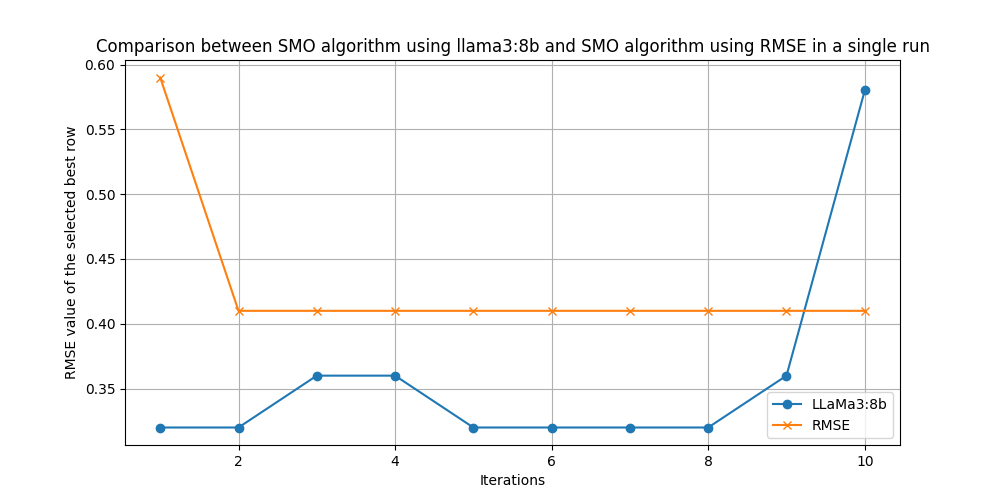
\includegraphics[page=1,width=0.5\textwidth]{llama3_8b_vs_rmse.png}
    \caption{Comparison between SMO with RMSE and SMO with LLMs on DataSet Auto 93 (Single Run) }
    \label{fig.3}
    \end{figure}
    
    In the Auto 93 dataset, we evaluated both SMO with Large Language Models (LLMs) and SMO with Root Mean Squared Error (RMSE), focusing on the final chosen best row's RMSE value as depicted in Figure \ref{fig.3}.
    
    During fine-tuning, we discovered that the most effective data adjustments originated from SMO with RMSE. We employed a comparison between optimal values derived from the SMO-RMSE algorithm with a random row as examples for few-shot learning with a large language model. This approach proved to be the valid in minimizing the RMSE values suggested by LLMs. Additionally, we encountered challenges with LLMs due to their inherent randomness and occasional logical errors in their outputs, such as incorrectly assessing the relative weights of objects.
    
    Moreover, while RMSE calculations depend not only on the target column but also on the overall data distribution, LLMs, despite being directed to base their responses on realistic scenarios, often do not align with RMSE standards, leading to larger RMSE values. However, LLMs offer a distinct advantage in recognizing the practical significance of data in real-world contexts.
    
    Despite efforts to provide reference ranges of data columns to improve LLMs' data comprehension, we observed no significant enhancements in their performance. We anticipate that increasing the iterations and integrating previous dialogues may improve LLMs' understanding of data distributions. However, utilizing LLM's memory capabilities remains challenging within the LangChain framework due to the substantial increase in prompt sizes it causes.
    
    \begin{figure}
    \centering
    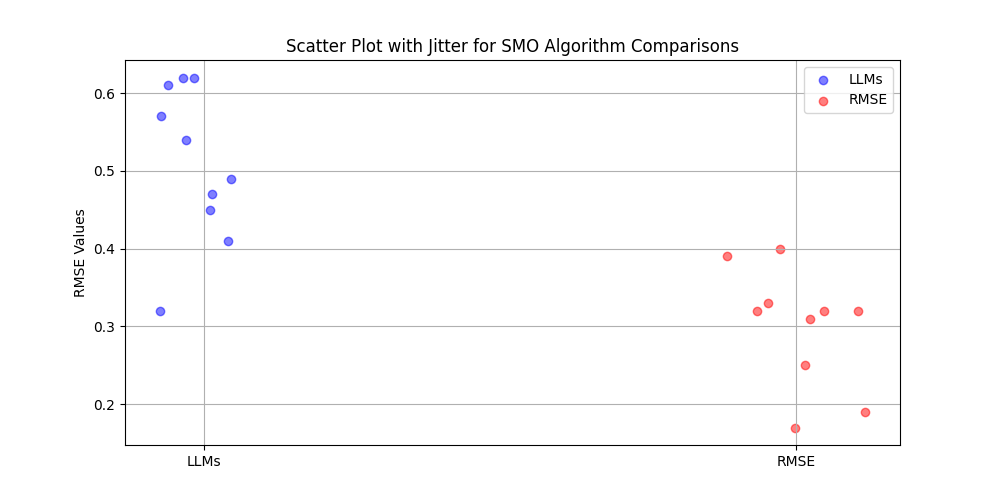
\includegraphics[page=1,width=0.5\textwidth]{llms_vs_rmse_10_run.png}
    \caption{Comparison between SMO with RMSE and SMO with LLMs on DataSet Auto 93 (10 Runs) }\label{fig.4}
    \end{figure}
    
    We conducted ten independent iterations of SMO using both RMSE and LLMs, as shown in Figure \ref{fig.4}. These experiments confirmed that while SMO with LLMs does not fully grasp the overall data distribution as RMSE does, it excels in contextual understanding and real-world applicability, unlike SMO with RMSE.
    
    \begin{figure}
    \centering
    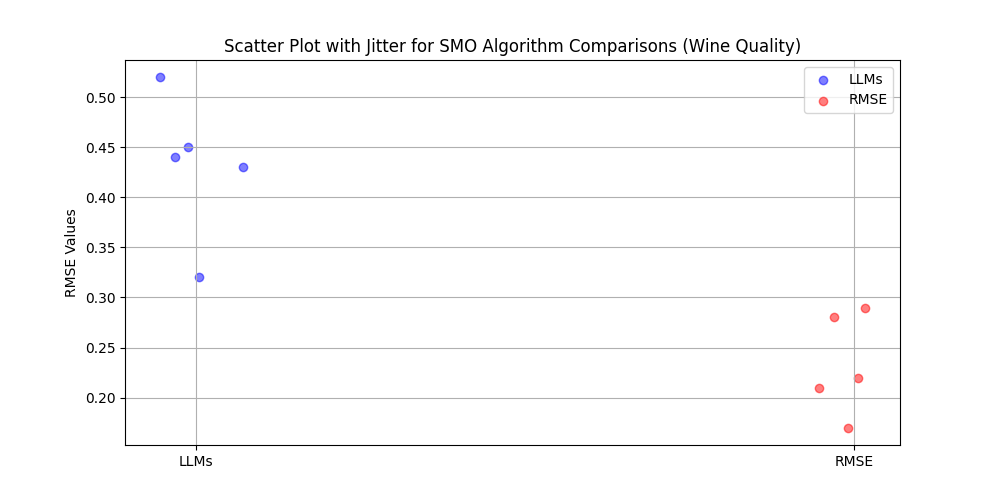
\includegraphics[page=1,width=0.5\textwidth]{llms_vs_rmse_5_run_wine.png}
    \caption{Comparison between SMO with RMSE and SMO with LLMs on DataSet Wine Quality (5 Runs) }\label{fig.5}
    \end{figure}
    
    Additionally, we applied the same experimental setup to the Wine Quality dataset with minimal adjustments, as shown in Figure \ref{fig.5}. Computational constraints limited us to five runs, highlighting the extensive demands of LLMs on processing resources. Notably, a GPU hardware failure during testing further complicated our experiments.
    
    In conclusion, while SMO with query recommendations via LLMs did not outperform SMO with RMSE in terms of RMSE evaluations, LLMs proved advantageous in terms of explainability, adaptability, and real-world relevance. The inherent challenges with LLMs, such as logical inconsistencies and their inability to fully comprehend the data distribution, were significant, yet their capacity to provide insightful, contextual explanations demonstrates their potential in applications where understanding complex scenarios is crucial.

\subsection{Statistical Methods}
For two primary algorithms compared in this paper - SMO with Language Learning Models (LLMs) and SMO with Root Mean Squared Error (RMSE), we conduct a Significance Test and an Effect Size Test.

\subsubsection{Significance Test using t-test}
For the Significance Test, we calculated the mean and variance for each method:
\[
\overline{X}_1 = 0.51, \quad s_1^2 = 0.0100 \quad \text{(Method LLMs)}
\]
\[
\overline{X}_2 = 0.30, \quad s_2^2 = 0.0058 \quad \text{(Method RMSE)}
\]

The t-test statistic was computed using the formula:
\[
t = \frac{\overline{X}_1 - \overline{X}_2}{\sqrt{\frac{s_1^2}{n_1} + \frac{s_2^2}{n_2}}} = \frac{0.51 - 0.30}{\sqrt{\frac{0.0100}{10} + \frac{0.0058}{10}}} \approx 5.283
\]

Where $n_1 = n_2 = 10$. The degrees of freedom for this test are \(df = n_1 + n_2 - 2 = 18\).

The p-value for the two-tailed test is calculated as:
\[
p = 2 \times \text{P}(T_{18} > |t|) \approx 5.05 \times 10^{-5}
\]

Since the p-value \((5.05 \times 10^{-5})\) is much less than the commonly used significance level of 0.05. This suggests that there is a statistically significant difference in RMSE between the two methods, with the SMO with LLMs having a higher average RMSE.

\subsection{Comparative Testing with Varying Numbers of Few-Shot Instances}

\begin{figure}
\centering
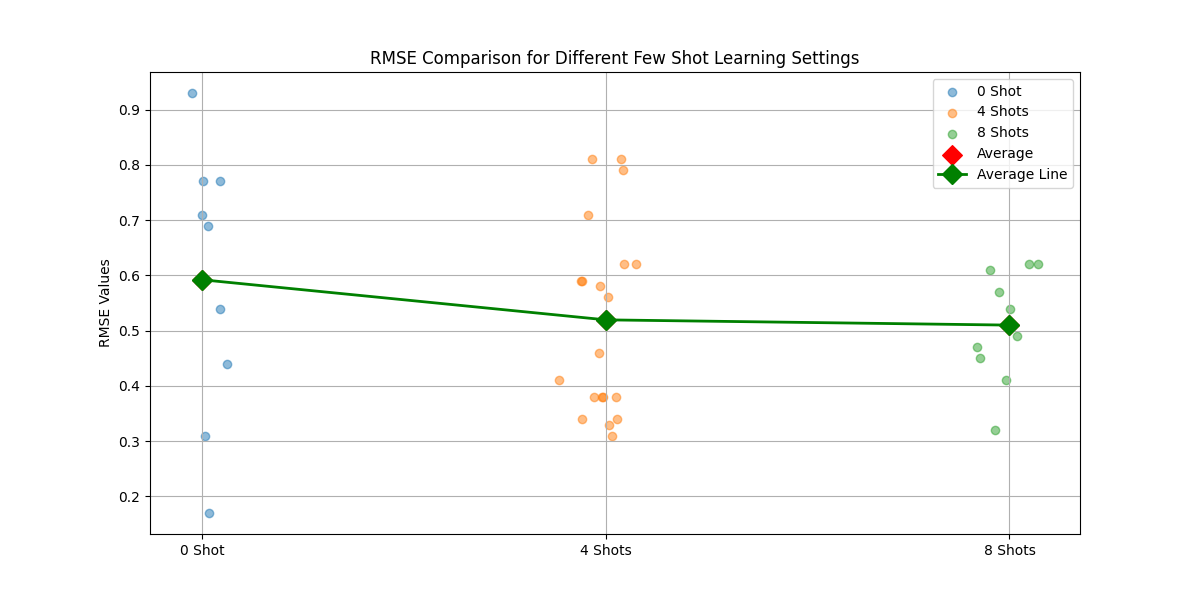
\includegraphics[page=1,width=0.5\textwidth]{few_shots.png}
\caption{Comparative testing with varying numbers of few-shot instances. \label{fig.6}}
\end{figure}

The experimental results depicted in Figure \ref{fig.6} demonstrate that as the number of few-shot instances increases, there is a corresponding improvement in the performance of SMO with LLMs. However, this enhancement in performance exhibits diminishing returns, with the most noticeable gains after approximately four shots. This trend suggests a limit to the effectiveness of adding more few-shot examples.

A noteworthy observation is that zero-shot learning may achieves some superior results compared to other few-shot configurations. This could be attributed to the unrestricted scope of response generation in zero-shot scenarios, which may enable broader contextual reasoning by the LLMs. Conversely, few-shot learning might constrain the LLMs' scope of thinking, thereby limiting their ability to leverage their extensive pre-trained knowledge. Another factor could be the inherent randomness introduced by zero-shot learning, which might more fitting unexpected query structures.

In conclusion, the impact of few-shot learning on enhancing LLM performance is significant but not linear. Increasing the number of few-shots does not invariably lead to better performance, especially as additional shots contribute to nearly linear increases in input token count for LLMs, resulting in increased response latency and computational cost. Therefore, based on our findings with the llama3 model, using four shots appears to be the optimal balance between performance improvement and computational efficiency. 

\subsection{Cost-performance considerations for various large language models}

\begin{figure}
\centering
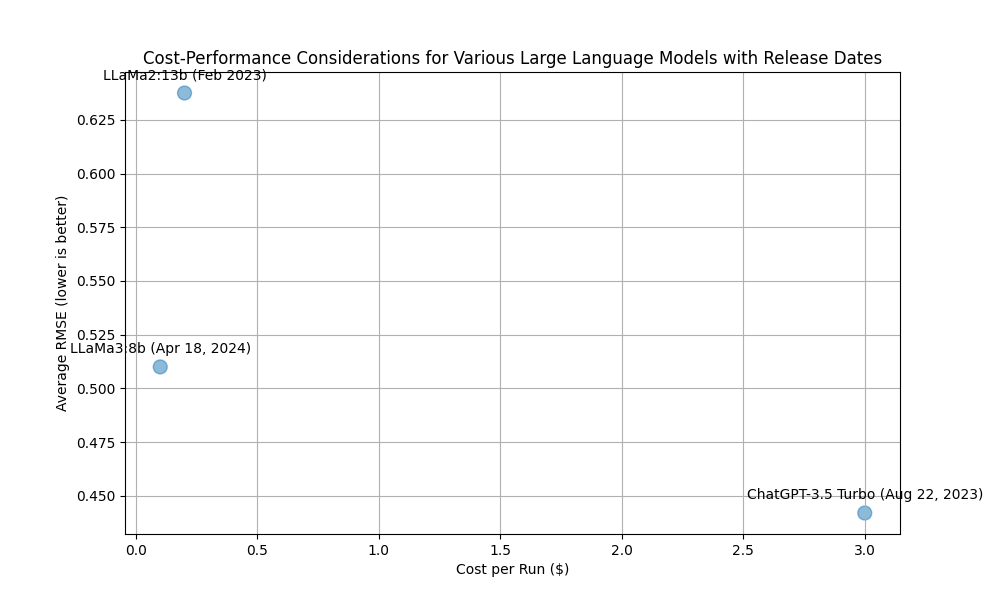
\includegraphics[page=1,width=0.5\textwidth]{cost_performance.png}
\caption{Cost-performance considerations for various large language models. }
\label{fig.7}
\end{figure}

As illustrated in Figure \ref{fig.7}, ChatGPT-3.5 Turbo, launched commercially last year, achieved the best performance in the SMO task among the models tested. However, it is also the most costly option, requiring \$15 to complete a pre-test plus 10 independent experiments. In addition to the financial cost, commercial models like ChatGPT-3.5 Turbo pose concerns regarding privacy, especially when dealing with sensitive datasets such as medical records. Despite these concerns, this model offers even faster response times through API calls compared to locally hosted solutions.

In contrast, open-source models, which can be run locally, may not perform as robustly as ChatGPT-3.5 Turbo, but they provide significant advantages in terms of cost and privacy, assuming the availability of suitable hardware (e.g., a graphics card). For example, LLaMA V3 has shown considerable improvement over its predecessor, LLaMA V2, operating with fewer tokens (8 billion compared to 13 billion) and reducing the performance gap between LLaMA with ChatGPT-3.5 Turbo by half.

In summary, the choice between commercial and open-source models involves a trade-off between performance and cost. While commercial models like ChatGPT-3.5 Turbo offer superior performance, they come with higher costs and potential privacy compromises. On the other hand, open-source models such as LLaMA V3 are progressively bridging the performance gap and offer benefits in terms of cost-efficiency and privacy due to their self-hostable nature.

\section{Discussion}
\label{sec:discussion}

\subsection{What was Learned}

\textbf{Large language models cannot solve all problems.} Despite their advanced capabilities, large language models (LLMs) still exhibit significant limitations when compared to traditional machine learning methods that can be explained mathematically. In the experiments involving SMO with RMSE, LLMs demonstrated a performance gap. A high RMSE value does not inherently imply inferiority in real-life scenarios; however, LLMs struggled to simulate the effectiveness of SMO with RMSE accurately. One major limitation is their restricted context capacity—for instance, the LLaMA v3 8B model has an input window of only 8K tokens, insufficient for handling extensive datasets. Although the SMO algorithm can mitigate this issue somewhat, the absence of memory for past inputs and responses significantly hampers LLMs' overall data comprehension. While fine-tuning might marginally improve performance, it demands substantial computational resources. Additionally, issues with debugging and model stability frequently arose during deployment, where models failed to respond as anticipated, and increasing few-shot instances did not fully resolve these issues.

Regarding hardware utilization, the LLaMA v3 8B model required about 6 GiB of memory on an NVIDIA 4070 SUPER TI GRAPHIC CARD graphics card, and its intense computational demands led to extended response times and software errors, reducing usability.

\subsection{Threats to Validity}

Constraints on resources and scope. The deployment of large language models is considerably resource-intensive. For instance, on the NVIDIA 4070 SUPER TI GRAPHIC CARD, an 8B model processes approximately 150 tokens per second. Given that each comparison prompt includes roughly 500 characters, each operation takes about three seconds.

In our experimental setup, the chosen parameters— \texttt{budget0}, \texttt{budget}, and \texttt{some} at 4, 16, and 0.5, respectively—meant that processing a dataset with 100 rows required about 16,000 iterations, equating to roughly an hour on a single GPU. Hence, we limited our study to two datasets. Without enhancements to the comparison or sorting algorithms, evaluating the efficiency of current models across more datasets, multiple iterations, and larger LLMs is challenging.

\subsection{Future Work}

Exploring more efficient sorting methods. The current inefficiency of the sorting algorithm constrains our ability to conduct comprehensive experiments within reasonable timeframes. Future research should focus on improving the sorting algorithm's efficiency. For instance, instead of comparing rows one by one, employing batch-wise sorting that allows LLMs to handle multiple lines simultaneously could significantly enhance efficiency.

More comprehensive evaluations. The capabilities of LLMs are promising, yet this study could not explore these due to the aforementioned inefficiencies. Future research should aim to:
\begin{itemize}
\item Compare SMO using RMSE and SMO using LLMs across a broader range of datasets.
\item Investigate variations in accuracy due to different LLMs and few-shot learning configurations.
\item Conduct a more detailed comparison of cost-performance ratios to chart the evolution of LLM capabilities.
\end{itemize}

\section{Conclusion}
\label{sec:conclusion}

This paper presented a comprehensive examination of Sequential Model Optimization (SMO) utilizing both traditional methods like Root Mean Square Error (RMSE) and innovative approaches involving Large Language Models (LLMs). Through rigorous testing on datasets like Auto 93 and Wine Quality, we explored the capabilities and limitations of these models in predictive analytics.

Our findings reveal that while LLMs offer advanced features and can handle complex real-world data interpretations, they still lag behind traditional methods in terms of accuracy as measured by RMSE. The inherent limitations of LLMs, particularly their restricted input capacity and lack of memory for past interactions, pose significant challenges in their application to extensive datasets. Despite these hurdles, the potential of LLMs to provide contextually rich insights and interpretations suggests a promising avenue for future research and application, particularly in scenarios where understanding nuanced real-world data is crucial.


In conclusion, while large language models have not yet surpassed traditional methods like RMSE in statistical optimization tasks, their evolving capabilities make them indispensable tools in the data scientist's toolkit. Future work should focus on overcoming the current limitations through more efficient algorithms, better model training techniques, and hardware optimizations to fully harness the power of LLMs in analytical applications. Moreover, further exploration into hybrid models that combine the interpretative power of LLMs with the precision of traditional statistical methods could yield solutions that are both powerful and practical for a wider range of applications.

% \appendices

% Appendixes, if needed, appear before the acknowledgment.

\section*{Acknowledgment}
I am grateful for Professor Tim Menzies' and Rahul Yadida's assistance towards me.




\begin{thebibliography}{00}

\bibitem{10352439}Long, D., Drylie, S., Ritschel, J. \& Koschnick, C. An Assessment of Rules of Thumb for Software Phase Management, and the Relationship Between Phase Effort and Schedule Success. {\em IEEE Transactions On Software Engineering}. \textbf{50}, 209-219 (2024)

\bibitem{yy} Yuanyuan Zhou, Keynote address, IEEE Automated Software Engineering conference, San Diego, California, USA, 2019. 

\bibitem{10.1145/2786805.2786852}Xu, T., Jin, L., Fan, X., Zhou, Y., Pasupathy, S. \& Talwadker, R. Hey, you have given me too many knobs!: understanding and dealing with over-designed configuration in system software. {\em Proceedings Of The 2015 10th Joint Meeting On Foundations Of Software Engineering}. pp. 307-319 (2015), https://doi.org/10.1145/2786805.2786852

\bibitem{10.1145/2961111.2962602}Han, X. \& Yu, T. An Empirical Study on Performance Bugs for Highly Configurable Software Systems. {\em Proceedings Of The 10th ACM/IEEE International Symposium On Empirical Software Engineering And Measurement}. (2016), https://doi.org/10.1145/2961111.2962602

\bibitem{9734271}Siegmund, N., Dorn, J., Weber, M., Kaltenecker, C. \& Apel, S. Green Configuration: Can Artificial Intelligence Help Reduce Energy Consumption of Configurable Software Systems?. {\em Computer}. \textbf{55}, 74-81 (2022)

\bibitem{791} Tim Menzies. Automated Software Engineering (2024 Spring) \emph{https://github.com/txt/aa24/tree/main}. 

\bibitem{Tawosi_2023} V. Tawosi, S. Alamir, and X. Liu, 
``Search-Based Optimisation of LLM Learning Shots for Story Point Estimation,'' 
in \emph{Lecture Notes in Computer Science}, 
Springer Nature Switzerland, 2023, pp. 123-129.
\textsc{doi}: \url{10.1007/978-3-031-48796-5_9}.

\bibitem{saparov2023testing}
Abulhair Saparov, Richard Yuanzhe Pang, Vishakh Padmakumar, Nitish Joshi, Seyed Mehran Kazemi, Najoung Kim, and He He.
\textit{Testing the General Deductive Reasoning Capacity of Large Language Models Using OOD Examples},
arXiv preprint arXiv:2305.15269, 2023.


\bibitem{radford2019language}
Alec Radford, Jeffrey Wu, Rewon Child, David Luan, Dario Amodei, and Ilya Sutskever.
\textit{Language Models are Unsupervised Multitask Learners},
OpenAI Blog, 2019.
URL: \url{https://cdn.openai.com/better-language-models/language_models_are_unsupervised_multitask_learners.pdf}

\bibitem{brown2020language}
Tom B. Brown, Benjamin Mann, Nick Ryder, Melanie Subbiah, Jared Kaplan, Prafulla Dhariwal, Arvind Neelakantan, Pranav Shyam, Girish Sastry, Amanda Askell, Sandhini Agarwal, Ariel Herbert-Voss, Gretchen Krueger, Tom Henighan, Rewon Child, Aditya Ramesh, Daniel M. Ziegler, Jeffrey Wu, Clemens Winter, Christopher Hesse, Mark Chen, Eric Sigler, Mateusz Litwin, Scott Gray, Benjamin Chess, Jack Clark, Christopher Berner, Sam McCandlish, Alec Radford, Ilya Sutskever, and Dario Amodei.
\textit{Language Models are Few-Shot Learners},
arXiv preprint arXiv:2005.14165, 2020.

\bibitem{devlin2018bert}
Jacob Devlin, Ming-Wei Chang, Kenton Lee, and Kristina Toutanova.
\textit{BERT: Pre-training of Deep Bidirectional Transformers for Language Understanding},
Proceedings of the 2019 Conference of the North American Chapter of the Association for Computational Linguistics (NAACL), 2018.
arXiv preprint arXiv:1810.04805.


\bibitem{chatgpt4}
OpenAI.
\textit{Introducing ChatGPT-4},
OpenAI Blog, 2023.
URL: \url{https://openai.com/blog/chatgpt-4}

\bibitem{claudeai}
Anthropic.
\textit{Claude: A helpful, honest, and harmless AI},
Anthropic Blog, 2023.
URL: \url{https://www.anthropic.com/claude}

\bibitem{llama}
Hugo Touvron, Thibaut Lavril, Gautier Izacard, Xavier Martinet, Marie-Anne Lachaux, Timothée Lacroix, Baptiste Rozière, Naman Goyal, Eric Hambro, Faisal Azhar, Aurélien Rodriguez, Armand Joulin, Edouard Grave, and Guillaume Lample.
\textit{LLaMA: Open and efficient foundation language models},
arXiv preprint arXiv:2302.13971, 2023.

\bibitem{gemma}
Google Research.
\textit{Introducing Gemma: Google's Generative Model for Multitask Applications},
Google AI Blog, 2023.
URL: \url{https://ai.googleblog.com/2023/gemma}

\bibitem{llamacpp}
Georgi Gerganov,
\textit{README for llama.cpp grammars}.
GitHub repository,
2024.
\url{https://github.com/ggerganov/llama.cpp/blob/master/grammars/README.md}.
Accessed: April 21, 2024.

\bibitem{auto_mpg_1993}
R. Quinlan (1993). Auto MPG. UCI Machine Learning Repository. Available: \url{https://doi.org/10.24432/C5859H}

\bibitem{cortez2009}
Paulo Cortez, A. Cerdeira, F. Almeida, T. Matos, and J. Reis (2009). 
\textit{Wine Quality}. 
UCI Machine Learning Repository. 
Available: \url{https://archive.ics.uci.edu/ml/datasets/Wine+Quality}

\end{thebibliography}
% \begin{IEEEbiography}[{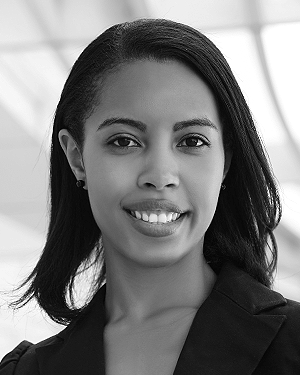
\includegraphics[width=1in,height=1.25in,clip,keepaspectratio]{a1.png}}]{First A. Author} (M'76--SM'81--F'87) and all authors may include 
% biographies. Biographies are often not included in conference-related
% papers. This author became a Member (M) of IEEE in 1976, a Senior
% Member (SM) in 1981, and a Fellow (F) in 1987. The first paragraph may
% contain a place and/or date of birth (list place, then date). Next,
% the author's educational background is listed. The degrees should be
% listed with type of degree in what field, which institution, city,
% state, and country, and year the degree was earned. The author's major
% field of study should be lower-cased. 

% The second paragraph uses the pronoun of the person (he or she) and not the 
% author's last name. It lists military and work experience, including summer 
% and fellowship jobs. Job titles are capitalized. The current job must have a 
% location; previous positions may be listed 
% without one. Information concerning previous publications may be included. 
% Try not to list more than three books or published articles. The format for 
% listing publishers of a book within the biography is: title of book 
% (publisher name, year) similar to a reference. Current and previous research 
% interests end the paragraph. The third paragraph begins with the author's 
% title and last name (e.g., Dr.\ Smith, Prof.\ Jones, Mr.\ Kajor, Ms.\ Hunter). 
% List any memberships in professional societies other than the IEEE. Finally, 
% list any awards and work for IEEE committees and publications. If a 
% photograph is provided, it should be of good quality, and 
% professional-looking. Following are two examples of an author's biography.
% \end{IEEEbiography}

% \begin{IEEEbiography}[{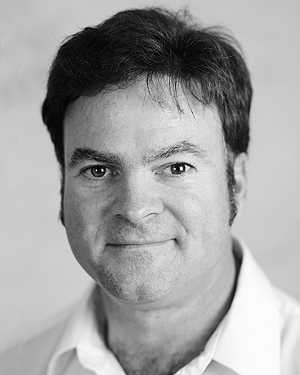
\includegraphics[width=1in,height=1.25in,clip,keepaspectratio]{a2.png}}]{Second B. Author} was born in Greenwich Village, New York, NY, USA in 
% 1977. He received the B.S. and M.S. degrees in aerospace engineering from 
% the University of Virginia, Charlottesville, in 2001 and the Ph.D. degree in 
% mechanical engineering from Drexel University, Philadelphia, PA, in 2008.

% From 2001 to 2004, he was a Research Assistant with the Princeton Plasma 
% Physics Laboratory. Since 2009, he has been an Assistant Professor with the 
% Mechanical Engineering Department, Texas A{\&}M University, College Station. 
% He is the author of three books, more than 150 articles, and more than 70 
% inventions. His research interests include high-pressure and high-density 
% nonthermal plasma discharge processes and applications, microscale plasma 
% discharges, discharges in liquids, spectroscopic diagnostics, plasma 
% propulsion, and innovation plasma applications. He is an Associate Editor of 
% the journal \emph{Earth, Moon, Planets}, and holds two patents. 

% Dr. Author was a recipient of the International Association of Geomagnetism 
% and Aeronomy Young Scientist Award for Excellence in 2008, and the IEEE 
% Electromagnetic Compatibility Society Best Symposium Paper Award in 2011. 
% \end{IEEEbiography}

% \begin{IEEEbiography}[{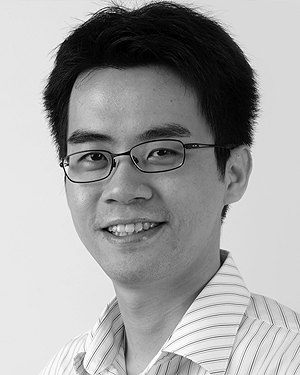
\includegraphics[width=1in,height=1.25in,clip,keepaspectratio]{a3.png}}]{Third C. Author, Jr.} (M'87) received the B.S. degree in mechanical 
% engineering from National Chung Cheng University, Chiayi, Taiwan, in 2004 
% and the M.S. degree in mechanical engineering from National Tsing Hua 
% University, Hsinchu, Taiwan, in 2006. He is currently pursuing the Ph.D. 
% degree in mechanical engineering at Texas A{\&}M University, College 
% Station, TX, USA.

% From 2008 to 2009, he was a Research Assistant with the Institute of 
% Physics, Academia Sinica, Tapei, Taiwan. His research interest includes the 
% development of surface processing and biological/medical treatment 
% techniques using nonthermal atmospheric pressure plasmas, fundamental study 
% of plasma sources, and fabrication of micro- or nanostructured surfaces. 

% Mr. Author's awards and honors include the Frew Fellowship (Australian 
% Academy of Science), the I. I. Rabi Prize (APS), the European Frequency and 
% Time Forum Award, the Carl Zeiss Research Award, the William F. Meggers 
% Award and the Adolph Lomb Medal (OSA).
% \end{IEEEbiography}

\EOD

\end{document}
